In this section, the results of the experiments of each step are discussed. Besides, different ideas and algorithms which are described in section \ref{sec:exp} are evaluated. At first, machine-learning-based experiments are presented. As machine learning feature engineering, requires multiple experiments to find best working predictors, there are many trials and errors for a variety of algorithms and ideas. Then, Deep learning models. are compared to machine learning models.
\section{Tokenizetion}
Tokenization of \textit{Hazm}, \textit{Stanford}, \textit{NLTK}, and \textit{BERT} are evaluated against each other manually. Every single difference is evaluated\footnote{All different cases during corpus tokenization by those 4 algorithms are gathered in \href{https://docs.google.com/document/d/1SlRBnoyLntLJ5yalWXZ1EqJ0wRj4DyiEMJdewkEkrTM/edit?usp=sharing}{here}}. Only three cases are presented as examples to compare each tokenizer's performance in figure \ref{fig:tekenres}. We need to remove particular words and patterns from the corpus so  it is important to find a tokenizer that distinguishes all words correctly. Besides, it shouldn't lose information while tokenizing and be as fast as possible. 

In figure \ref{fig:tekenres}, unsuitable tokens are highlighted  blue. There isn't any flawless algorithm. As BERT is  subwords, there are some UNK tokens and wrongly words broken by BERT tokenizing. For example figure \ref{fig:tekenres}, part (b) blue highlighted word is broken into two pieces wrongly. Strength of \textit{Stanford} tokenizer, is that consider connected pronoun individually. But sometimes \text{Stanford} wrongly breaks an original word with a wrong assumption that the desired word has a connected pronoun. Figure \ref{fig:tekenres}, part (c) is a sample on wrong separating pronoun and at part (b), pronouns are separated correctly. It can be seen in figure \ref{fig:tekenres} \textit{Hazm} performance is highly similar to \textit{NLTK}. The only difference is that in contrast \textit{NLTK}, Hazm separates numbers and punctuation in the corpus (Figure \ref{fig:tekenres}, part (a)). 

\begin{figure}%
	\centering
	\subfloat[\centering]{{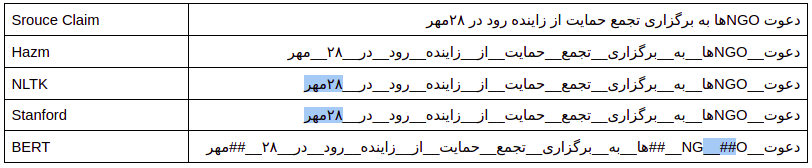
\includegraphics[width=16cm]{statistics/tokenizer/1.png} }}%
	\qquad
	\subfloat[\centering ]{{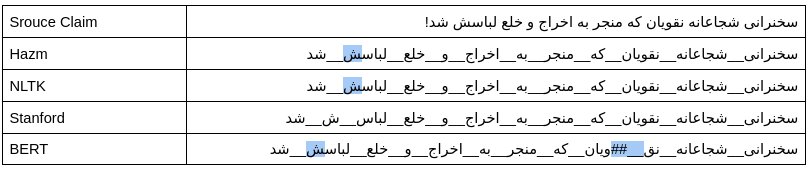
\includegraphics[width=16cm]{statistics/tokenizer/2.png} }}%
	\qquad
	\subfloat[\centering]{{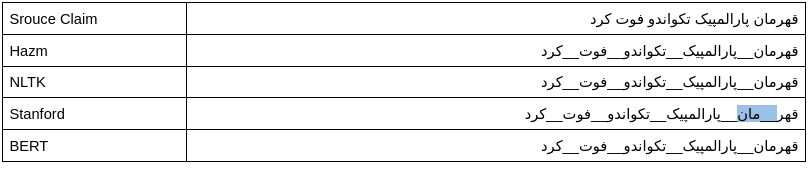
\includegraphics[width=16cm]{statistics/tokenizer/3.png} }}%
	\caption{Comparison performance of \textit{Hazm}, \textit{Stanford}, \textit{NLTK} and \textit{BERT} tokenizers.}%
	\label{fig:tekenres}%
\end{figure}

Besides, the duration of tokenizing for each tokenizer is compared in figure \ref{fig:tokentime}. While \textit{Hazm} is the fastest words tokenizer among evaluated algorithms, \textit{Stanford} tokenizer last vastly longer. According to all pieces of evidence, \textit{Hazm} tokenizer is the best tokenizer for this task.

\begin{figure}%
	\centering
	{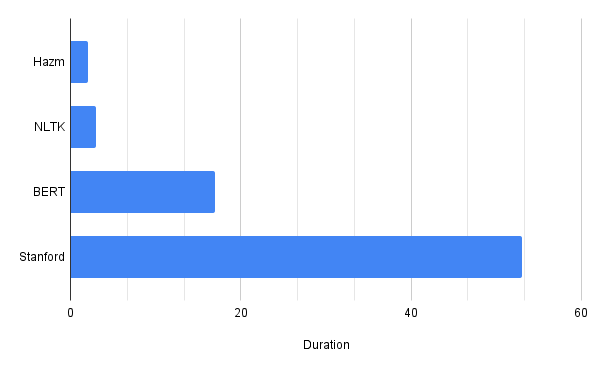
\includegraphics[width=12.5cm]{statistics/tokenizer/duration.png} }
	\caption{Comparison duration of tokenizing algorithm on \cite{stance_persian} dataset.}%
	\label{fig:tokentime}%
\end{figure}


\section{Stop-Words}
Three sets of stop words is evaluated it this section. \cite{stance_persian} contains 1255 words which include wide a range of parts of speech. In contrast, NonVerbal\footnote{Gathered by \href{github.com/kharazi/persian-stopwords}{Kharazi}} stop words set include 158 words and it doesn't support any verb. In the new version of stop-words, 18 stop words are removed from the Nonverval set. This set is called \textit{shortened} and 82 new words are added. Finally, the \textit{Extended} version contains 233 words. To evaluate the performance of each stop-words sets, all desired features with Tf-iDF as word representation after removing particular stop words are fed into an SVM (\cite{svc}) model. To having a fair comparison, non-targeting removing the stop-words is also compared. 

It can be inferred from figure \ref{fig:stopwords} that the list of stop words which is used by \cite{stance_persian} is ignoring valuable data and it is even better not to remove stop words. Nonverbal stop-words achieve higher accuracy on stance detection. Through, whether removing or adding words from Nonverbal (\textit{shortened} version) didn't improve results. Altogether, Nonverbal list of stop-words, performs the best in this task.

\begin{figure}%
	\centering
	{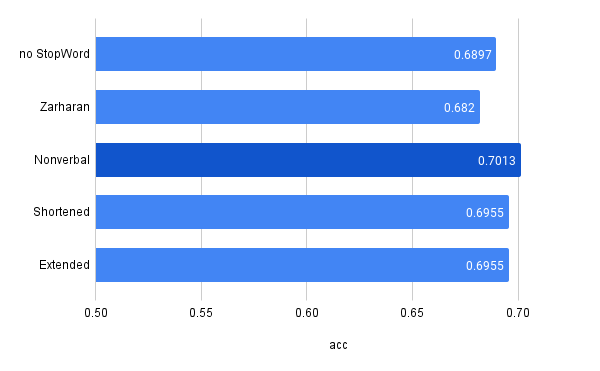
\includegraphics[width=12.5cm]{statistics/AccuracyScore.png} }
	\caption{Comparison accuracy of SVM model with different configuration of stop words.}%
	\label{fig:stopwords}%
\end{figure}

\section{Word Representation}
In this section, Bow (\cite{bow}), TF-iDF, and Word2Vec (\cite{word2vec}) performances are compared by SVM machine learning algorithm in the stance detection task. According to figure \ref{fig:wordrep} Tf-iDF performs the best in comparison to BoW and Word2Vec in order to represent words.
\begin{figure}%
	\centering
	{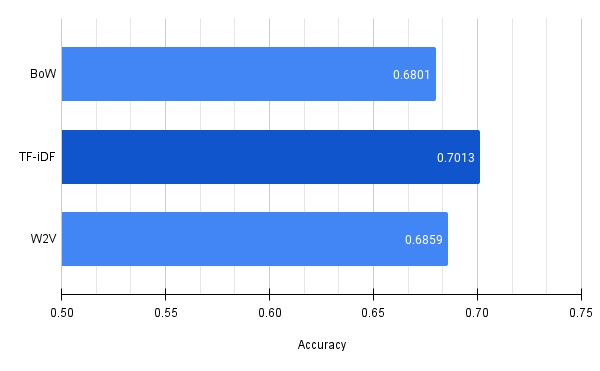
\includegraphics[width=12.5cm]{statistics/WordRep.png} }
	\caption{Comparison SVM model with Bow, TF-iDF and Word2Vec word representaion algorithms.}%
	\label{fig:wordrep}%
\end{figure}

\section{Predictors}
\label{sec:predictors}
Different combinations of calculated predictor are run to find out that which set of predictors performs better. Desired predictors are Similarity, RootDistance, IsQuestion, HasTwoParts and Polarity. In this Section, both SVM (\cite{svc}) and RandomForest (\cite{randomforest}) results are considered in evaluation to have a more accurate analysis.

Firstly, both models are trained on the corpus representation by TF-iDF without any other predictor. Then, each predictor is added into TF-iDF vector to evaluate their effectiveness individually, and finally, all features together are fed to models. According to table \ref{tlb:predictors}, Similarity and ImportantWords have the highest positive effect respectively, on both accuracy (\ref{eq:acc}) and f1-score (\ref{eq:f1}). Similarity score has improved accuracy 15 to 17 percent and ImportantWords has improved SVM accuracy by almost 4 percent. Though, predictors such as IsQuestion, HasTwoParts, and Polarity don't have a significant effect on results, using them all together boost total accuracy and f1-score. 

Due to figure \ref{tlb:predictors}, using RootDistance, IsQuestion, and HasTwoParts individually decreases accuracy, so models are also trained with two other variations. Though IsQuestion, HasTwoParts, and polarity don't have a positive effect individually, using them with Similarity, ImportantWrods, and polarity boost accuracy. On the other hand, removing RootDistance from All predictors mode whether have a negligible effect or improves accuracy. 

According to previous comparisons and evaluation inferred from table \ref{tlb:predictors}, the best predictors to use for stance detection task is the combination of Similarity, ImportantWords, IsQuestion, HasTwoParts, and Polarity predictors in addition to TD-iDF as the corpus representer, altogether.


\begin{table}[]
	\centering
	\caption{Comparison of accuracy and F1-score with different combinations of predictors for both SVM and Random Forest classifiers.}
	\setlength{\extrarowheight}{13pt}%
	\begin{tabular*}{350pt}{@{\extracolsep{\fill}}| l | l | l | l | l |}
		\hline
		\multicolumn{1}{|c|}{} & \multicolumn{2}{l|}{SVM} & 
		\multicolumn{2}{l|}{RandomForest}  \\ \cline{2-5} 
		
		\multicolumn{1}{|c|}{\multirow{-2}{*}{\begin{tabular}[c]{@{}c@{}}Predictors\\  Model\end{tabular}}}         & Acc.    & F1.    & Acc.    & F1.    \\ \cline{1-1}
		
		\hline
		
		\multicolumn{1}{|c|}{TF-iDF only} & 51.83   & 51.90   & 52.79   & 54.00   \\ \cline{1-1}
		\hline
		+ Similarity      		& 66.85   & 66.71   & 68.78   & 67.88   \\ \cline{1-1}
		\hline
		+ Root Distance   		& 51.25   & 51.50   & 49.71   & 50.52   \\ \cline{1-1}
		\hline
		+ Important Words 		& 56.64   & 56.94   & 52.98   & 52.49   \\ \cline{1-1}
		\hline
		+ Is Question     		& 51.63   & 51.79   & 51.63   & 52.70   \\ \cline{1-1}
		\hline
		+ Has Two Parts   		& 51.83   & 51.90   & 50.28   & 50.87   \\ \cline{1-1}
		\hline
		+ Polarity        		& 52.21   & 52.50   & 52.40   & 53.25   \\ \cline{1-1}
		\hline
		+ All                   & 69.74   & 69.75  & 69.36   & 68.75   \\ \cline{1-1}
		\hline
		+ All - Root Distance   & 69.74   & 69.69   & \textbf{70.71}   & \textbf{70.28}   \\ \hline
		+ Similarity + ImportantWords   & 69.74   & 69.69   & 67.82  & 67.02  \\ \hline
	\end{tabular*}
	\label{tlb:predictors}
\end{table}

\section{Machine Learning}
In this section, each Gaussian Naive Bayes, SVM, Linear SVC, Random Forest, and Logistic Regression parameters are tuned on stance detection task with respect to chosen predictors in the previous section (\ref{sec:predictors}). In the next step, the performance of models is compared to each other.

\subsection{SVM}
Three SVM classifier tuned parameters  are Kernel, Regularization parameter (C) and degree of polynomial kernel. Evaluated kernels are RBF, Polynomial and Sigmoid. According to figure \ref{fig:svm}, Sigmoid works weak for this task. Each polynomial kernel behaves differently due value of the regularization parameter. Polynomial with degrees 2 and 3 performs better than 1 and 4. Linear polynomial may be so simple and SVM is not good enough to classify stance with polynomial with degree 4. RBF, Polynomial degree 3 behave similarly due to the regularization parameter changes. 

The best configuration for SVM classifier is using RBF as the kernel with regularization parameter equal to 2.5 confirming figure \ref{fig:svm}. Learning procedure and details of each model training exist in this project GitHub repository\footnote{Different SVM configuration training details \href{https://github.com/mahsaghn/stance\_detection/tree/main/selected\_outputs/machinelearning/svm}{[here]}.}.

\begin{figure}% 
	\centering
	{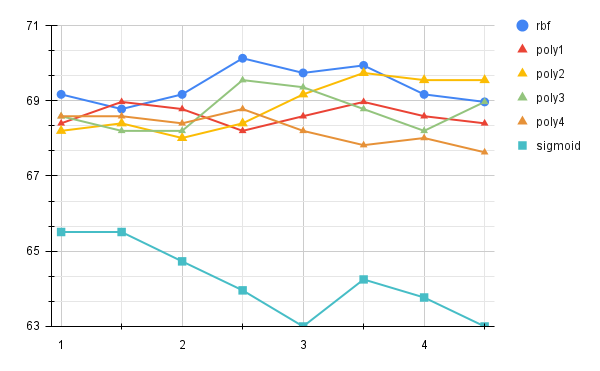
\includegraphics[width=12.5cm]{statistics/svm.png} }
	\caption{Tuning SVM model parameters with TF-iDF representaion algorithms}%
	\label{fig:svm}%
\end{figure}

\subsection{Linear SVC}
Linear Support Vector Machine Classifier algorithm, loss function and Regularization parameters are tuned with penalty equals to \textit{l2}. Figure \ref{fig:linearsvm} illustrates comparison between linear svm models with loss functions equal to Hinge or Squared Hinge, and tuned SVM algorithm. Hinge loss function has scored better performance than Squared Hinge. When Squared Hing is used as loss function, as the Regularization parameter increases, accuracy score decrease. Though Regularization parameter don't have significant effect on accuracy score when loss is equal to Hinge. In conclusion, due to figure \ref{fig:linearsvm} Best configuration is for Hinge loss and Regularization parameter equals to 1.0. 
\begin{figure}% 
	\centering
	{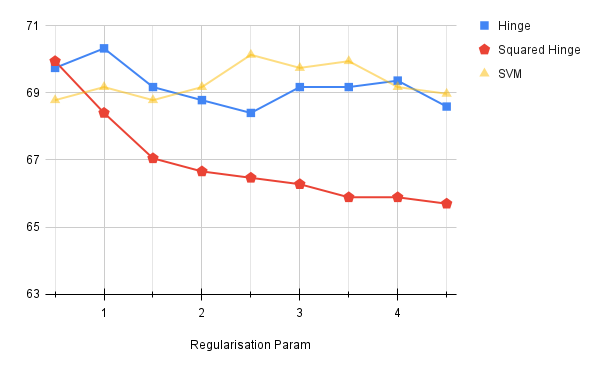
\includegraphics[width=12.5cm]{statistics/linearsvm.png} }
	\caption{Tuning LinearSVC model parameters with TF-iDF representaion algorithms.}%
	\label{fig:linearsvm}%
\end{figure}
\subsection{Random Forest}
Random Forest criterion, maximum number of feature in each decision tree and number of tree are evaluated. Figure \ref{fig:randomforest} illustrates effect of number of tree in forest on accuracy among different configuration. Accuracy of models increase on average by adding more trees into the forest. Besides, \textit{gini} algorithm performs better than \textit{entropy} to measure quality of splits. Also, three different upper bound is considered for number of features when looking for a split. No boundary, \textit{sqrt} of total feature and \textit{log2} of total feature. According to figure \ref{fig:randomforest} don't applying any boundary leads to better accuracy in average. Furthermore, as the boundary get tighten average performance decreases. 

Best configuration for Random Forest machine learning model in this task is using \textit{gini} algorithm to evaluate splitting quality, not applying any boundary on number of features and having 125 decision tree in the forest. 
\begin{figure}% 
	\centering
	{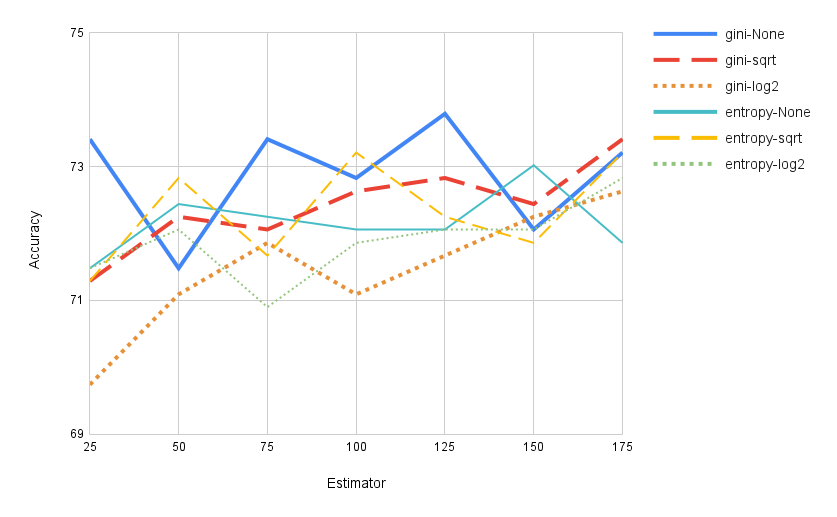
\includegraphics[width=12.5cm]{statistics/randomforest.png} }
	\caption{Random Forest machine learning model different configuration on stance detection task. Type of line presents type of boundary applied on each model. Solid line, dash line and doted line stands for no boundary, sqrt of total feature and log2 of total feature respectively.}%
	\label{fig:randomforest}%
\end{figure}
\subsection{Logistic Regression}
Many experiments are designed to evaluate behavior of Logistic Regression models. 	 \textit{Elasticnet} (Equation \ref{eq:logisel}) penalty algorithm which is used in penalization procedure, used for \textit{saga} solver and \textit{l2} penalty algorithm is used for \textit{sag}, \textit{lbfgs}, and \textit{newton-cg} solvers. 

\textit{Elasticnet} has a $\rho$ parameter which determines portion of using $l1$ to $l2$ penalty in \textit{saga} solver. Figure \ref{fig:logistic1} illustrate effect of $\rho$ values from $0$ to $0.9$ on accuracy of stance detection. Besides, models with regression parameter from $0.5$ to $4.5$ are evaluated from determined $\rho$ range. It can be inferred from figure \ref{fig:logistic1} that $\rho$ parameter doesn't have significant effect on accuracy of the model. While, regression parameter between $1$ and $2.5$ clearly results in higher accuracy rather than external range. It can be also inferred from figure \ref{fig:logistic2} which illustrates effect of regression parameter on stance classification accuracy. Models with different value of $\rho$ behave similarly and best performances happens when regression parameter is between $1$ and $2.5$.  
\begin{figure}% 
	\centering
	{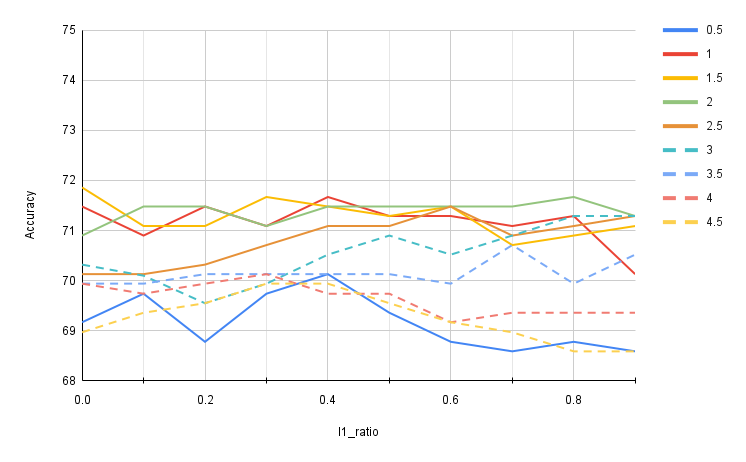
\includegraphics[width=12.5cm]{statistics/logistic_elastic1.png} }
	\caption{Effect of $\rho$ parameter of \textit{elasticnet} penalty on stance detection task.}%
	\label{fig:logistic1}%
\end{figure}
\begin{figure}% 
	\centering
	{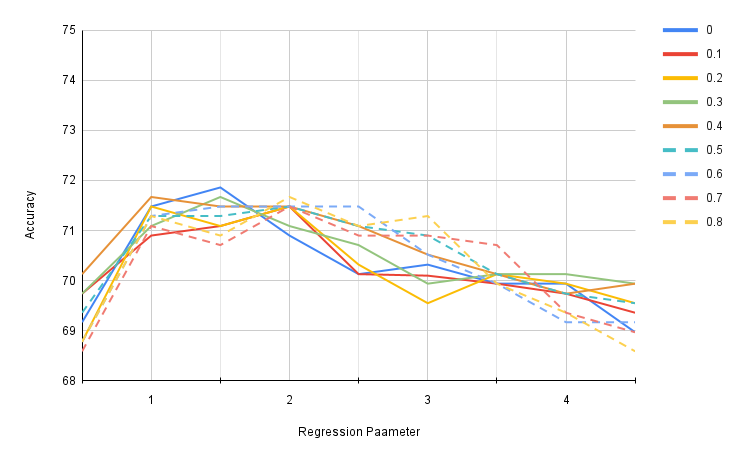
\includegraphics[width=12.5cm]{statistics/logistic_elastic2.png} }
	\caption{Effect of regression parameter of \textit{elasticnet} penalty on stance detection task.}%
	\label{fig:logistic2}%
\end{figure}

Another variants of Logistic Regression setup is to use $l2$ penalty with desired solver algorithms. Figure \ref{fig:logistic3} compares best \textit{saga} solver with \textit{sag}, \textit{lbfgs}, and \textit{newton-cg}. The Logistic Regression with \textit{lbfgs} solver and regression parameter equals to 1.5 has recorded the highest accuracy. 
\begin{figure}% 
	\centering
	{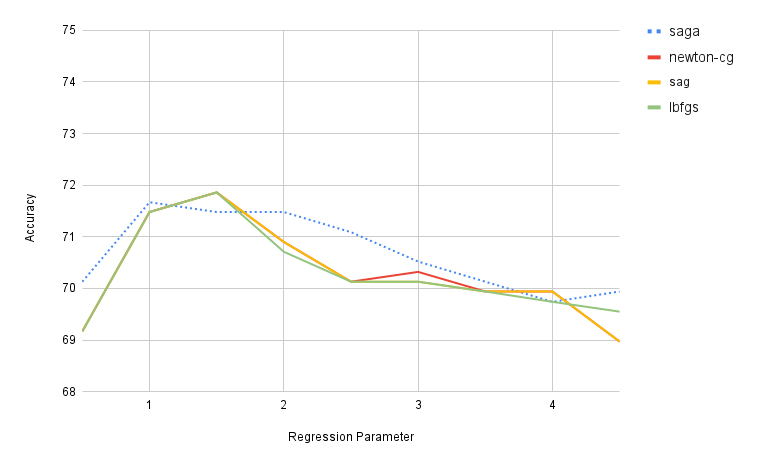
\includegraphics[width=12.5cm]{statistics/logistic1.png} }
	\caption{}%
	\label{fig:logistic3}%
\end{figure}

\subsection{Comparison}
In previous sections parameters of each SVM, LinearSVC, Random Forest, and Logistic Regression models are tuned. In this section models with desired parameters has run 5 times each to have more reliable results and comparison. Average accuracy and highest accuracy recorded in tuning phase, compared in figure \ref{fig:all}. The highest achievable accuracy with machine learning models to classify stance of a claim towards the headline of a news article is 74.01\%.
\begin{figure}% 
	\centering
	{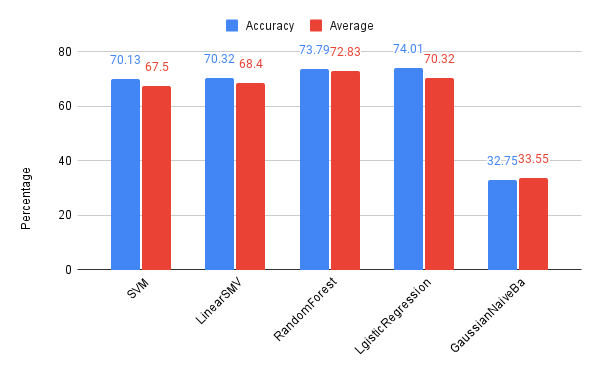
\includegraphics[width=12.5cm]{statistics/machinlearning.png} }
	\caption{Comparison SVM model with Bow, TF-iDF and Word2Vec word representation algorithms.}%
	\label{fig:all}%
\end{figure}
\section{Dataset Balancing}
Firstly, ADASYN, SMOTE, SVMSMOTE, BorderLineSmote, and RandomOverSampler oversampling methods are applied on the \cite{stance_persian} dataset. Each method is evaluated against five desired machine learning models. Red sereis in figure \ref{fig:balanc} stands for the accuracy of models, associated with the \cite{stance_persian} dataset. LinearSVC, LogisticRegresion, and GaussianNaibeBayes are not compatible with any oversampling method. Though, ADASYN oversampling method has increased these two model accuracy 5 percent on average. 

At the second step, dataset is extend by the ParsFever (\cite{parsfever}) dataset. Though, number of samples are increased accuracy is obviously decreased, but the GaussianNB model. This may happens that data sources from each dataset are totally different and headlines in ParsFever are much longer than the \cite{stance_persian} dataset.
\begin{figure}% 
	\centering
	{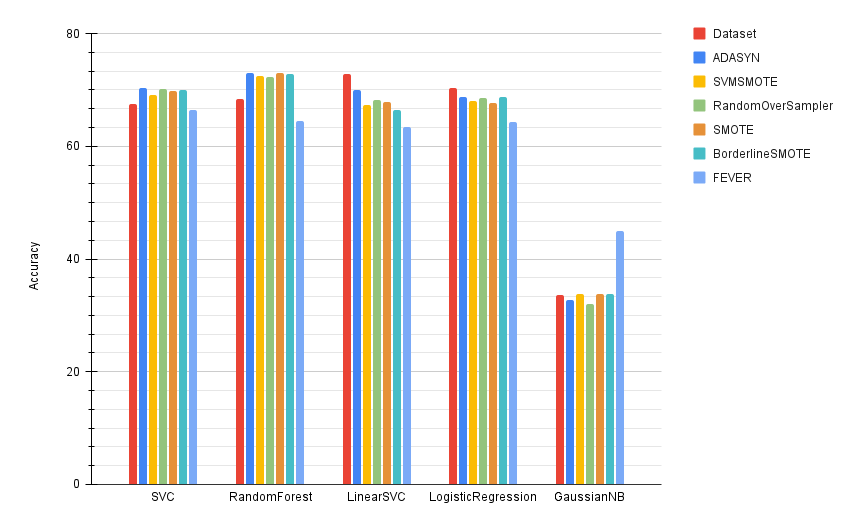
\includegraphics[width=14.5cm]{statistics/balancing.png} }
	\caption{Comparison SVM model with Bow, TF-iDF and Word2Vec word representation algorithms.}%
	\label{fig:balanc}%
\end{figure}

\section{Deep Learning}
Pre-trained BERT model is used at the top of the model, then two Dense layers and finally a Dense including 4 neuron to classify stance is considered for end-to-end system. Each epochs lasts about 26 seconds in training procedure. Figure \ref{fig:deep} illustrates the model training procedure. In comparison to machine learning models, the deep learning model has boosted the accuracy of head to claim stance detection by 10 percent. 

BERT-based model has learned for 20 epochs. Validation loss has stated to increase since epoch 11 and validation accuracy hasn't changed considerably then. Best validation accuracy has converged on 80.92\% on the headline-to-claim dataset. 

ParsBert-based model has learned for 20 epochs. Best validation accuracy has converged on 81.11\% on the headline-to-claim dataset. In comparison to machine learning algorithm, deep learning algorithm has enhanced about 10\% accuracy.

Though, best recorded ALBERT language model on 20 epochs is at most 70.52\% on accuracy score. Figure \ref{fig:deep}, part (e) and (f) is illustrated training procedure.

Among these three alternative of BERT algorithm, PasrBERT based model has recorded best accuracy score with 81.11\% accuracy on stance prediction.  
\begin{figure}%
	\centering
	\subfloat[\centering]{{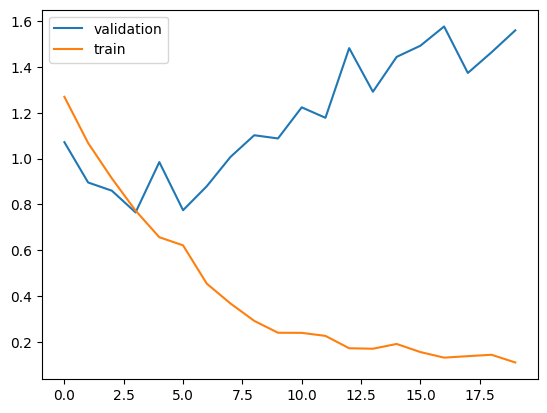
\includegraphics[width=6cm]{statistics/deep/bert_loss.png} }}%
	\qquad
	\subfloat[\centering]{{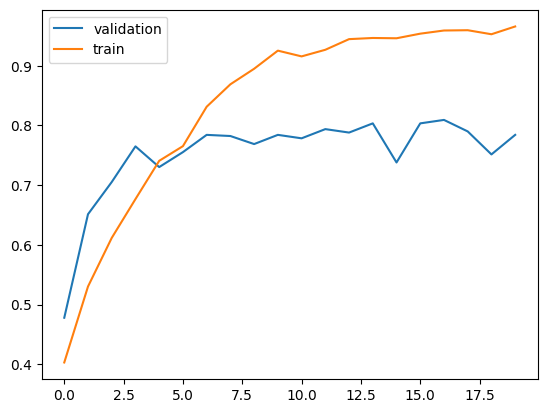
\includegraphics[width=6cm]{statistics/deep/bert_acc.png} }}%
	\qquad
	\subfloat[\centering]{{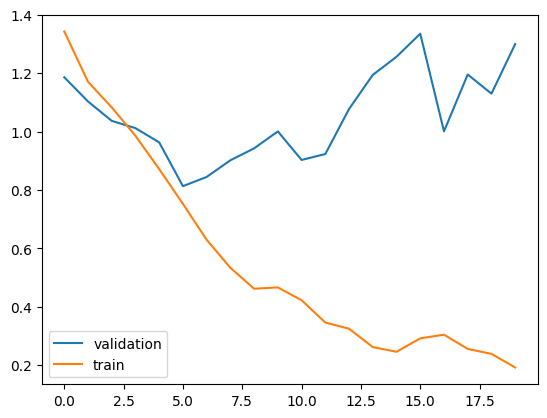
\includegraphics[width=6cm]{statistics/deep/parsbert_loss.png} }}%
	\qquad
	\subfloat[\centering]{{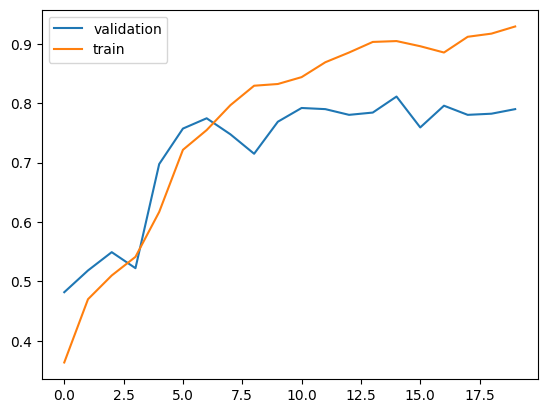
\includegraphics[width=6cm]{statistics/deep/parsbert_acc.png} }}%
	\qquad
	\subfloat[\centering]{{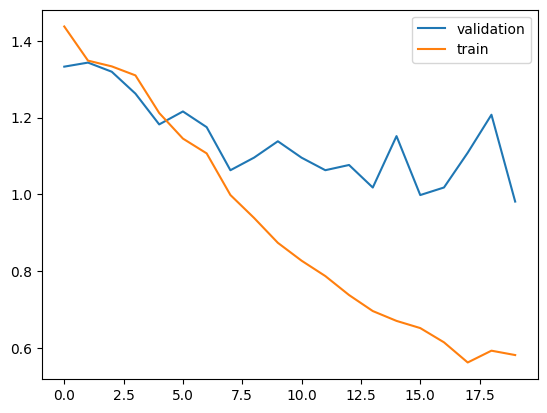
\includegraphics[width=6cm]{statistics/deep/albert_loss.png} }}%
	\qquad
	\subfloat[\centering]{{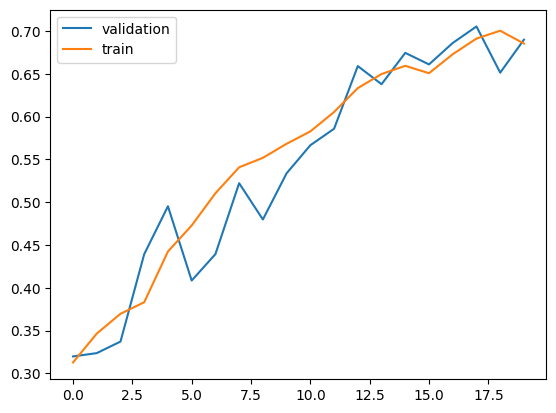
\includegraphics[width=6cm]{statistics/deep/albert_acc.png} }}%
	
	
	\caption{Deep learning procedure on the headline-to-claim stance detection task. Left figures illustrate loss score and right figures illustrate accuracy score of train and test data during training procedure. (a, b) Pre-trained language model based on Google's BERT (\cite{parsbert}) on Persian corpus (c, d) Pre-trained monolingual language model based on ParsBERT (\cite{parsbert}) on Persian corpus. (e, f) Pre-trained language model based on ALBERT (\cite{albert}) on Persian corpus}%
	\label{fig:deep}%
\end{figure}


\section{Fake News}
BERT-based model is concatenated with features which are described in section \ref{sec:fakenews} then feed to an three-layer MLP model as the classifier. ADASYN oversampling method is also used to deal with imbalanced classes. Figure \ref{fig:fakenews} illustrates training procedure before oversampling and after oversampling the dataset. After oversampling, the trained model accuracy is equal to 100\%.